% !TEX encoding = UTF-8 Unicode

\documentclass[aspectratio=169]{beamer}
\usepackage[utf8]{inputenc}

%% BIB
\usepackage[
  style=authoryear,
  backend=biber,
  url=false,
  maxcitenames=2,
  uniquename=false,
  uniquelist=false
]{biblatex}
\addbibresource{nems.bib}
\addbibresource{yeast.bib}

%% GRAPHICS

\usepackage{graphicx}
\graphicspath{{images/},{figures/}}
\usepackage{tikz}

%% COLORS
\definecolor{UWRed}{HTML}{C5050C}
\definecolor{StrongBlue}{HTML}{3F8FD2}
\definecolor{StrongGreen}{HTML}{36C88E}
\definecolor{StrongRed}{HTML}{9B0000}
\definecolor{MyC}{HTML}{009999}
\definecolor{MyM}{HTML}{990099}
\definecolor{MyY}{HTML}{999900}
\definecolor{MyR}{HTML}{990000}
\definecolor{MyG}{HTML}{009900}
\definecolor{MyB}{HTML}{000099}
\definecolor{ActionRed}{HTML}{990000}

%% SLIDE COLOR SETTINGS
\setbeamercolor{structure}{fg=UWRed}
\setbeamercolor{title page}{fg=white}
\setbeamercolor{title}{fg=white}

%% RM NAV SYMBOLS
\setbeamertemplate{navigation symbols}{}

%% FONTS
\setbeamerfont{title}{size=\huge\bfseries}

%% DRAWING
\usetikzlibrary{fit,calc,arrows,arrows.meta,decorations.pathreplacing,decorations.text,decorations.pathmorphing,backgrounds,fit,positioning,shapes,chains,topaths,matrix}

\def\firstcircle{(90:0.3cm) circle (0.6cm)}
\def\secondcircle{(210:0.3cm) circle (0.6cm)}
\def\thirdcircle{(330:0.3cm) circle (0.6cm)}

\tikzset{%
  link/.style={->,>=angle 45,semithick},
  var/.style={circle,draw,minimum size=1.5em,align=center, inner sep=0pt, anchor=center},
  text block/.style={rectangle, rounded corners, draw=#1, fill=white, thick, text width=5em, align=center},
  thick arrow/.style={
     -{Triangle[angle=120:1pt 1]},
%     -Triangle,
     line width=2em, 
     draw=SoftBlue
  },
  arrow label/.style={
    text=white,
    font=\sf,
    align=center
  },
  set mark/.style={
    insert path={
      node [midway, arrow label, node contents=#1]
    }
  },
  set vertical mark/.style={
    insert path={
      node [midway, arrow label, node contents=#1, rotate=-90]
    }
  },
  colormap/.pic={code={    
    \fill[MyC] \firstcircle;
    \fill[MyM] \secondcircle;
    \fill[MyY] \thirdcircle;
    
    % C+M, C+Y
    \begin{scope}
      \clip \firstcircle;
      \fill[MyB] \secondcircle;
      \fill[MyG] \thirdcircle;
    \end{scope}
    
    % M+Y, K
    \begin{scope}
      \clip \secondcircle;
      \fill[MyR] \thirdcircle;
      \clip \firstcircle;
      \fill[black] \thirdcircle;
    \end{scope}
    
    \draw[thick, white] \firstcircle;
    \draw[thick, white] \secondcircle;
    \draw[thick, white] \thirdcircle;
    
    \node[white] at (90:0.6cm) {\scriptsize\bf 1};
    \node[white] at (210:0.6cm) {\scriptsize\bf 2};
    \node[white] at (330:0.6cm) {\scriptsize\bf 3};
  }},
  onslide/.code args={<#1>#2}{
    \only<#1>{\pgfkeysalso{#2}}
  }
}

%% LOGO on slides
\logo{\begin{tikzpicture}[overlay]
  \node[anchor=north east,inner sep=0] at (0,86mm) {
\includegraphics[height=10mm]{SMPH_color-flush.pdf}};
\end{tikzpicture}}

%% CONTENT BEGINS

\title{Context-Specific Nested Effect Models}
\subtitle{RECOMB 2018, Paris}
\author{\textbf{Yuriy Sverchkov} \and Elisha Yi-Hsuan Ho \and Audrey P. Gash \and Mark Craven}
\institute{University of Wisconsin--Madison}
\date{April 24, 2018}

\begin{document}

  {
    \usebackgroundtemplate{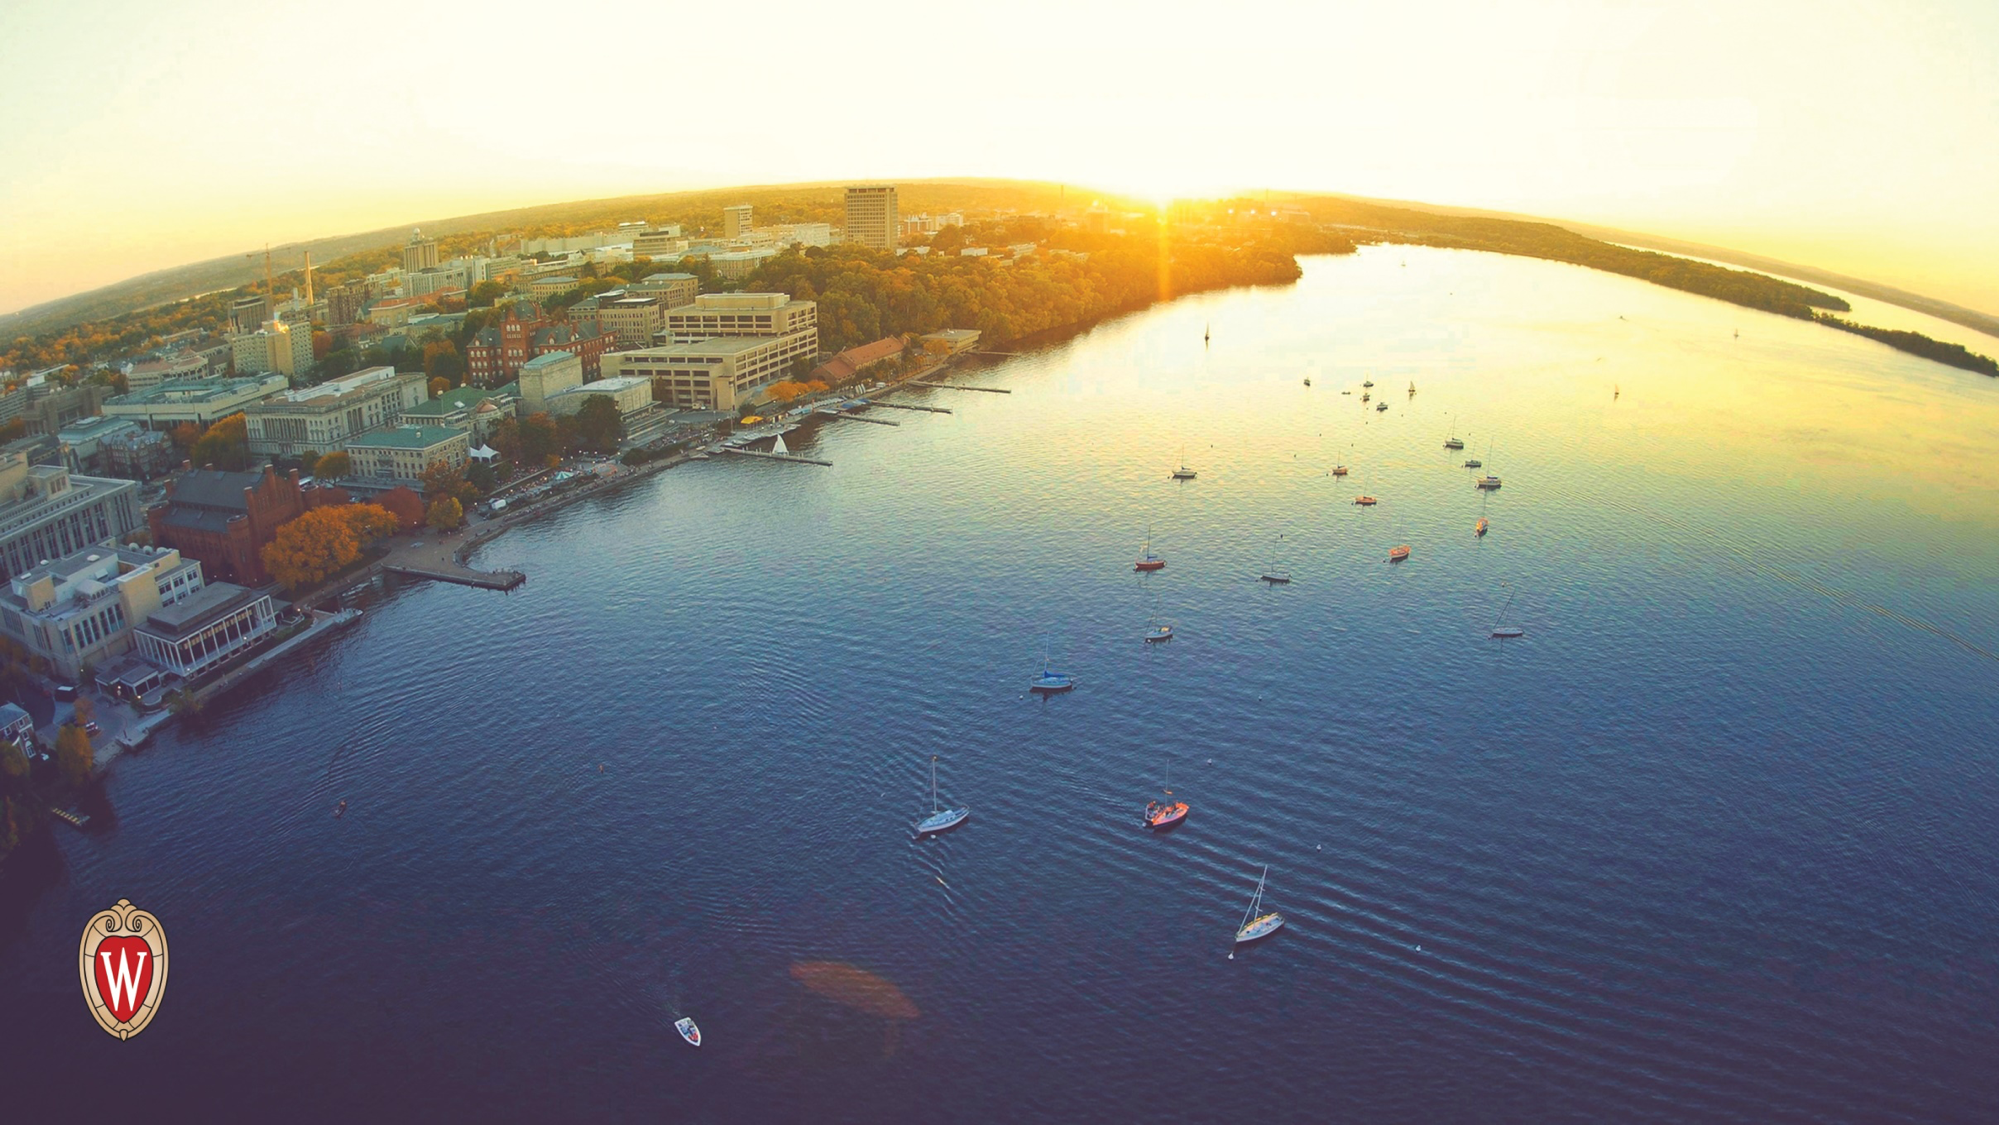
\includegraphics[width=\paperwidth]{UW-lake.png}}
    \begin{frame}[plain]
      \vskip4cm
      \titlepage
    \end{frame}
  }

\begin{frame}{Context-specific biological networks}
\centering
\begin{tikzpicture}[very thick, ampersand replacement=\&]

 \matrix (mr) [matrix of nodes, nodes={fill=black!20, onslide=<1>{text=white, fill=ActionRed} }, column sep=0.5em] at (0,-2cm) {
  $e_1$ \& $e_2$ \& $e_3$ \& $e_4$ \& $e_5$ \& $e_6$ \\
 };

 {\color<1>{StrongBlue}
  \node[var] (a) at (0,5mm) {A};
  \node[var] (b1) at (-1cm,-5mm) {B};
  \node[var] (c) at (1cm,-5mm) {C};
 
  \draw[link] (a) to (b1);
  \draw[link] (a) to (c);
 
  \draw[link] (b1) to (mr-1-1);
  \draw[link] (b1) to (mr-1-2);
  \draw[link] (a) to (mr-1-3);
  \draw[link] (a) to (mr-1-4);
  \draw[link] (c) to (mr-1-5);
  \draw[link] (c) to (mr-1-6);
 }
  
 \uncover<2->{
  
  \matrix (ml) [matrix of nodes, nodes={fill=black!20, onslide=<2>{text=white, fill=ActionRed}}, column sep=0.5em] at (4cm, -2cm) {
    $e_7$ \& $e_8$ \\
  };

  {\color<2>{ActionRed}
   \node[var] (b2) at (4cm,0) {B};

   \draw[link] (b2) to (ml-1-1);
   \draw[link] (b2) to (ml-1-2);
  
  
   \node[draw, ellipse, fit=(b2) (ml),decoration={snake, amplitude=0.5mm},decorate] (organelle) {};
  }
 }
 
 \node[draw, ellipse, fit=(a) (b1) (mr) (organelle), double, double distance=1mm] (cell) {};

 \uncover<1>{
  \node[text block,anchor=south,text width=8cm] at (cell.south) {\textbf{Task:} infer {\color{StrongBlue} causal relationships} from \color{ActionRed}{observed high-dimensional phenotypes (\textbf{effects})}};
 }
 \uncover<2>{
  \node[text block,anchor=south,text width=8cm] at (cell.south) {\textbf{Context-specificity:} the same actors can have different relationships in different \textbf{\color{ActionRed} contexts}.};
 }

\end{tikzpicture}
\end{frame}
  
%%% FRAMEBREAK %%%

\begin{frame}{Uncovering biological networks}
  \centering
  \begin{tikzpicture}[very thick, ampersand replacement=\&]

    \matrix (es) [matrix of nodes, column sep = 0.5em] at (0,-2cm) {
      \& |[fill=StrongGreen,onslide={<4,5>{fill=StrongRed}}]|$e_1$
      \&  |[fill=StrongGreen,onslide={<4,5>{fill=StrongBlue}}]|$e_2$
      \& |[fill=StrongRed,onslide={<4,5>{fill=StrongBlue}}]|$e_3$
      \& |[fill=StrongRed,onslide={<4>{fill=StrongBlue}}]|$e_4$
      \& |[fill=StrongBlue]|$e_5$
      \& |[fill=StrongGreen,onslide={<4,6>{fill=StrongBlue}}]|$e_6$
      \& |[fill=StrongBlue,onslide={<4,6>{fill=StrongGreen}}]|$e_7$
      \& |[fill=StrongRed,onslide={<4,6>{fill=StrongGreen}}]|$e_8$ \\
    };
    
    \uncover<3->{
      \node[var] (a) at (0,0) {A};
      \node[var] (b) at (-1cm, -1cm) {B}; 
      \node[var] (c) at (1cm, -1cm) {C};

      \draw[link,onslide=<4>{ActionRed}] (a) to (b);
      \draw[link,onslide=<4>{ActionRed}] (a) to (c);
      \draw[link,{onslide=<4,5>{ActionRed}}] (b) to (es-1-2);
      \draw[link,{onslide=<4,5>{ActionRed}}] (b) to (es-1-3);
      \draw[link,{onslide=<4,5>{ActionRed}}] (b) to (es-1-4);
      \draw[link,onslide=<4>{ActionRed}] (a) to (es-1-5);
      \draw[link,{onslide=<4,6>{ActionRed}}] (c) to (es-1-7);
      \draw[link,{onslide=<4,6>{ActionRed}}] (c) to (es-1-8);
      \draw[link,{onslide=<4,6>{ActionRed}}] (c) to (es-1-9);
    }
    
    \only<4>{
      \draw[line width=1mm, ActionRed] (a.north west) to (a.south east);
      \node[anchor=west, ActionRed] at (a.east) {$\Delta$};
    }
    \only<5>{
      \draw[line width=1mm, ActionRed] (b.north west) to (b.south east);
      \node[anchor=west, ActionRed] at (b.east) {$\Delta$};
    }
    \only<6>{
      \draw[line width=1mm, ActionRed] (c.north west) to (c.south east);
      \node[anchor=west, ActionRed] at (c.east) {$\Delta$};
    }
    
    \node[draw, ellipse, very thick, fit=(a) (b) (c) (es), double, double distance=1mm] (cell) {};

  \matrix (d) [below=5mm of cell, matrix of nodes, nodes={}] {
  \& $e_1$ \& $e_2$ \& $e_3$ \& $e_4$ \& $e_5$ \& $e_6$ \&  $e_7$ \& $e_8$ \\
  WT \& |[fill=StrongGreen]| \&  |[fill=StrongGreen]| \& |[fill=StrongRed]| \& |[fill=StrongRed]| \& |[fill=StrongBlue]| \& |[fill=StrongGreen]| \& |[fill=StrongBlue]| \& |[fill=StrongRed]| \\
  $A\Delta$ \& |[fill=StrongRed]| \&  |[fill=StrongBlue]| \& |[fill=StrongBlue]| \& |[fill=StrongBlue]| \& |[fill=StrongBlue]| \& |[fill=StrongBlue]| \& |[fill=StrongGreen]| \& |[fill=StrongGreen]| \\
  $B\Delta$ \& |[fill=StrongRed]| \&  |[fill=StrongBlue]| \& |[fill=StrongBlue]| \& |[fill=StrongRed]| \& |[fill=StrongBlue]| \& |[fill=StrongGreen]| \& |[fill=StrongBlue]| \& |[fill=StrongRed]| \\
  $C\Delta$ \& |[fill=StrongGreen]| \&  |[fill=StrongGreen]| \& |[fill=StrongRed]| \& |[fill=StrongRed]| \& |[fill=StrongBlue]| \& |[fill=StrongBlue]| \& |[fill=StrongGreen]| \& |[fill=StrongGreen]| \\
 };
  \uncover<1>{ \node[fill=white,fit=(d-2-1) (d-1-9), inner sep=0] {};}
  \uncover<4->{ \node[fill=white,opacity=0.5, fit=(d-2-1) (d-2-9), inner sep=0] {};}
  \node[fill=white,onslide=<4>{opacity=0},onslide=<5-6>{opacity=0.5},fit=(d-3-1) (d-3-9), inner sep=0] {};
  \node[fill=white,onslide=<5>{opacity=0},onslide=<6>{opacity=0.5},fit=(d-4-1) (d-4-9), inner sep=0] {};
  \uncover<-5>{ \node[fill=white,fit=(d-5-1) (d-5-9), inner sep=0] {};}
  
 %   \uncover<7>{
 %     \node[anchor=south, fill=white] at (d.north) {High-dimensional phenotype};
 %   }
    \uncover<1>{
     \node[text block,text width=8cm,below=0mm of cell] {\textbf{Effects} are things we can measure: high-dimensional phenotypes, e.g., metabolomics, proteomics, etc.};
    }
  \end{tikzpicture}
\end{frame}

%%% FRAMEBREAK

\begin{frame}{High-dimensional knockout screens}

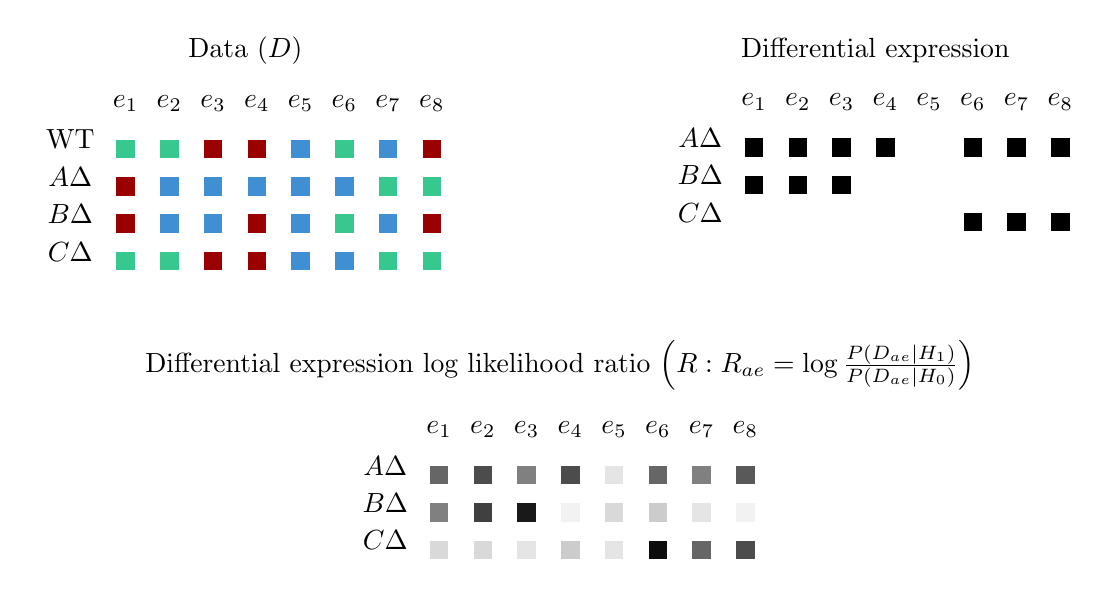
\begin{tikzpicture}[very thick, ampersand replacement=\&]

 \node (data) {Data ($D$)};
 \matrix (dmx) [anchor=north, matrix of nodes] at (data.south) {
  \& $e_1$ \& $e_2$ \& $e_3$ \& $e_4$ \& $e_5$ \& $e_6$ \&  $e_7$ \& $e_8$ \\
  WT \& |[fill=StrongGreen]| \&  |[fill=StrongGreen]| \& |[fill=StrongRed]| \& |[fill=StrongRed]| \& |[fill=StrongBlue]| \& |[fill=StrongGreen]| \& |[fill=StrongBlue]| \& |[fill=StrongRed]| \\
  $A\Delta$ \& |[fill=StrongRed]| \&  |[fill=StrongBlue]| \& |[fill=StrongBlue]| \& |[fill=StrongBlue]| \& |[fill=StrongBlue]| \& |[fill=StrongBlue]| \& |[fill=StrongGreen]| \& |[fill=StrongGreen]| \\
  $B\Delta$ \& |[fill=StrongRed]| \&  |[fill=StrongBlue]| \& |[fill=StrongBlue]| \& |[fill=StrongRed]| \& |[fill=StrongBlue]| \& |[fill=StrongGreen]| \& |[fill=StrongBlue]| \& |[fill=StrongRed]| \\
  $C\Delta$ \& |[fill=StrongGreen]| \&  |[fill=StrongGreen]| \& |[fill=StrongRed]| \& |[fill=StrongRed]| \& |[fill=StrongBlue]| \& |[fill=StrongBlue]| \& |[fill=StrongGreen]| \& |[fill=StrongGreen]| \\
  };
 \uncover<2->{
	\node (de) at (8,0) {Differential expression};
	\matrix (demx) [anchor=north, matrix of nodes] at (de.south) {
  \& $e_1$ \& $e_2$ \& $e_3$ \& $e_4$ \& $e_5$ \& $e_6$ \&  $e_7$ \& $e_8$ \\
  $A\Delta$ \& |[fill=black]| \&  |[fill=black]| \& |[fill=black]| \& |[fill=black]| \& \& |[fill=black]| \& |[fill=black]| \& |[fill=black]| \\
  $B\Delta$ \& |[fill=black]| \& |[fill=black]| \& |[fill=black]| \& \& \& \& \& \& \& \& \\
  $C\Delta$ \& \& \& \& \& \& |[fill=black]| \& |[fill=black]| \& |[fill=black]| \\
 };
 }
 \uncover<3->{
	\node (lode) at (4,-4) {Differential expression log likelihood ratio $\left( R : R_{ae} = \log \frac{ \mathbb P( D_{ae} | H_1 ) }{ \mathbb P( D_{ae} | H_0 ) } \right)$};
	\matrix (lodemx) [anchor=north, matrix of nodes] at (lode.south) {
  \& $e_1$ \& $e_2$ \& $e_3$ \& $e_4$ \& $e_5$ \& $e_6$ \&  $e_7$ \& $e_8$ \\
  $A\Delta$ \& |[fill=black!60]| \&  |[fill=black!70]| \& |[fill=black!50]| \& |[fill=black!70]| \& |[fill=black!10]| \& |[fill=black!60]| \& |[fill=black!50]| \& |[fill=black!65]| \\
  $B\Delta$ \& |[fill=black!50]| \& |[fill=black!75]| \& |[fill=black!90]| \& |[fill=black!5]| \& |[fill=black!15]| \& |[fill=black!20]| \& |[fill=black!10]| \& |[fill=black!5]| \\
  $C\Delta$ \& |[fill=black!15]| \& |[fill=black!15]| \& |[fill=black!10]| \& |[fill=black!20]| \& |[fill=black!10]| \& |[fill=black!95]| \& |[fill=black!60]| \& |[fill=black!70]| \\
 };
 }
\end{tikzpicture}

\end{frame}

%%% FRAMEBREAK %%%

\begin{frame}{Nested effect model (NEM)}

\begin{columns}
\column{0.5\textwidth}

\begin{tikzpicture}[very thick, ampersand replacement=\&]

 {\color{StrongGreen}
  \matrix (es) [anchor=north, matrix of nodes] at (de.south) {
  \& $e_1$ \& $e_2$ \& $e_3$ \& $e_4$ \& $e_5$ \& $e_6$ \&  $e_7$ \& $e_8$ \\
  $A\Delta$ \& |[fill]| \&  |[fill]| \& |[fill]| \& |[fill]| \& \& |[fill]| \& |[fill]| \& |[fill]| \\
  $B\Delta$ \& |[fill]| \& |[fill]| \& |[fill]| \& \& \& \& \& \& \& \& \\
  $C\Delta$ \& \& \& \& \& \& |[fill]| \& |[fill]| \& |[fill]| \\
 };
  \node[anchor=north] at (es.south) {Effect matrix $F$};
 }
 
 \node[var, above=3 of es] (a) {A};
 \node[var, below left=of a] (b) {B}; 
 \node[var, below right=of a] (c) {C};
 
 {\color{StrongBlue}
 \draw[link] (a) to (b);
 \draw[link] (a) to (c);
 }
 {\color{StrongRed}
 \draw[link] (b) to (es-1-2);
 \draw[link] (b) to (es-1-3);
 \draw[link] (b) to (es-1-4);
 \draw[link] (a) to (es-1-5);
 \draw[link] (c) to (es-1-7);
 \draw[link] (c) to (es-1-8);
 \draw[link] (c) to (es-1-9);
 }

\end{tikzpicture}

\column{0.4\textwidth}
\uncover<2>{
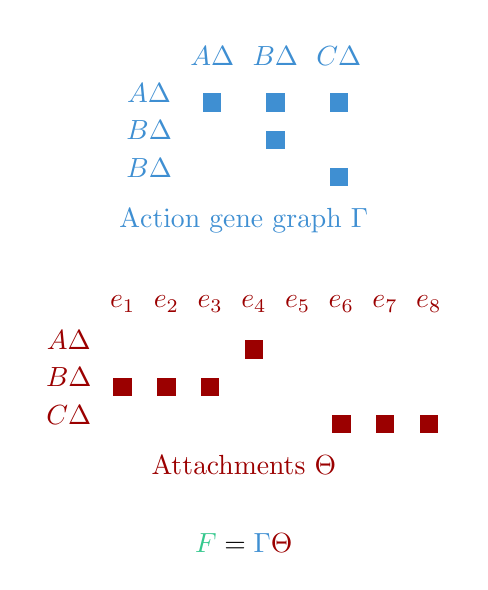
\begin{tikzpicture}[very thick, ampersand replacement=\&]

 {\color{StrongBlue} 
 \matrix (gamma) [matrix of nodes] {
  \& $A\Delta$ \& $B\Delta$ \& $C\Delta$ \\
  $A\Delta$ \& |[fill]| \&  |[fill]| \& |[fill]| \\
  $B\Delta$ \& \& |[fill]| \& \\
  $B\Delta$ \& \& \&  |[fill]| \\
 };
 \node[anchor=north] at (gamma.south) {Action gene graph $\Gamma$};
 }
 
 {\color{StrongRed}
 \matrix (theta) [below=of gamma, matrix of nodes] {
  \& $e_1$ \& $e_2$ \& $e_3$ \& $e_4$ \& $e_5$ \& $e_6$ \&  $e_7$ \& $e_8$ \\
  $A\Delta$ \& \& \& \& |[fill]| \& \& \& \& \\
  $B\Delta$ \& |[fill]| \& |[fill]| \& |[fill]| \& \& \& \& \& \& \& \& \\
  $C\Delta$ \& \& \& \& \& \& |[fill]| \& |[fill]| \& |[fill]| \\
 };
 \node[anchor=north] at (theta.south) {Attachments $\Theta$};
 }
 
 \node (formula) [below=of theta] {${\color{StrongGreen} F} = {\color{StrongBlue} \Gamma} {\color{StrongRed}\Theta}$};

\end{tikzpicture}
}
\end{columns}

{\small \textcite{Markowetz01012005}}
\end{frame}

%%% FRAMEBREAK %%%

\begin{frame}{Context-specific nested effect model (CSNEM)}
\centering
\begin{tikzpicture}[very thick, ampersand replacement=\&]

 \node[var] (a) at (0,5mm) {A};
 \node[var] (b1) at (-1cm,-5mm) {B};
 \node[var] (c) at (1cm,-5mm) {C};
 \node[var] (b2) at (4cm,0) {B};

 \matrix (mr) [matrix of nodes, nodes={fill=black!20, onslide=<3>{white,fill=ActionRed}}, column sep=0.5em] at (0,-2cm) {
   |[onslide=<4>{white,fill=ActionRed}]| $e_1$ \& |[onslide=<4>{white,fill=ActionRed}]| $e_2$ \& $e_3$ \& $e_4$ \& $e_5$ \& $e_6$ \\
 };
 
 \matrix (ml) [matrix of nodes, nodes={fill=black!20, onslide=<4>{white,fill=ActionRed}}, column sep=0.5em] at (4cm, -2cm) {
   $e_7$ \& $e_8$ \\
 };
 
 \draw[link,onslide=<3>{ActionRed}] (a) to (b1);
 \draw[link,onslide=<3>{ActionRed}] (a) to (c);
 
 \draw[link,onslide=<3-4>{ActionRed}] (b1) to (mr-1-1);
 \draw[link,onslide=<3-4>{ActionRed}] (b1) to (mr-1-2);
 \draw[link,onslide=<3>{ActionRed}] (a) to (mr-1-3);
 \draw[link,onslide=<3>{ActionRed}] (a) to (mr-1-4);
 \draw[link,onslide=<3>{ActionRed}] (c) to (mr-1-5);
 \draw[link,onslide=<3>{ActionRed}] (c) to (mr-1-6);
 \draw[link,onslide=<4>{ActionRed}] (b2) to (ml-1-1);
 \draw[link,onslide=<4>{ActionRed}] (b2) to (ml-1-2);
 
 \node[draw, ellipse, fit=(b2) (ml),decoration={snake, amplitude=0.5mm},decorate] (organelle) {};
 \node[draw, ellipse, fit=(a) (b1) (mr) (organelle), double, double distance=1mm] (cell) {};

 \uncover<2->{
 \matrix (mx) [matrix of nodes, fill=white, below=2cm of cell.center, nodes ={black}] {
  \& $e_1$ \& $e_2$ \& $e_3$ \& $e_4$ \& $e_5$ \& $e_6$ \&  $e_7$ \& $e_8$ \\
  \color<3>{ActionRed} $A\Delta$ \& |[fill, onslide=<3>{fill=ActionRed}]| \&  |[fill=black, onslide=<3>{fill=ActionRed}]| \& |[fill=black, onslide=<3>{fill=ActionRed}]| \& |[fill=black, onslide=<3>{fill=ActionRed}]| \& |[fill=black, onslide=<3>{fill=ActionRed}]| \& |[fill=black, onslide=<3>{fill=ActionRed}]| \& \& \\
  \color<4>{ActionRed} $B\Delta$ \& |[fill=black, onslide=<4>{fill=ActionRed}]| \& |[fill=black, onslide=<4>{fill=ActionRed}]| \& \& \& \& \& |[fill=black, onslide=<4>{fill=ActionRed}]| \& |[fill=black, onslide=<4>{fill=ActionRed}]| \\
  $C\Delta$ \& \& \& \& \& |[fill=black]| \& |[fill=black]| \& \& \\
 };
 }
 
 \only<3>{
   \draw[very thick, ActionRed] (a.north west) to (a.south east);
   \node[anchor=west, ActionRed] at (a.east) {$\Delta$};
 }

 \only<4>{
   \draw[very thick, ActionRed] (b1.north west) to (b1.south east);
   \node[anchor=west, ActionRed] at (b1.east) {$\Delta$};
   \draw[very thick, ActionRed] (b2.north west) to (b2.south east);
   \node[anchor=west, ActionRed] at (b2.east) {$\Delta$};
 }


\end{tikzpicture}
\end{frame}

%%% FRAMEBREAK %%%

\begin{frame}{CSNEM as a mixture of NEMs}
\centering
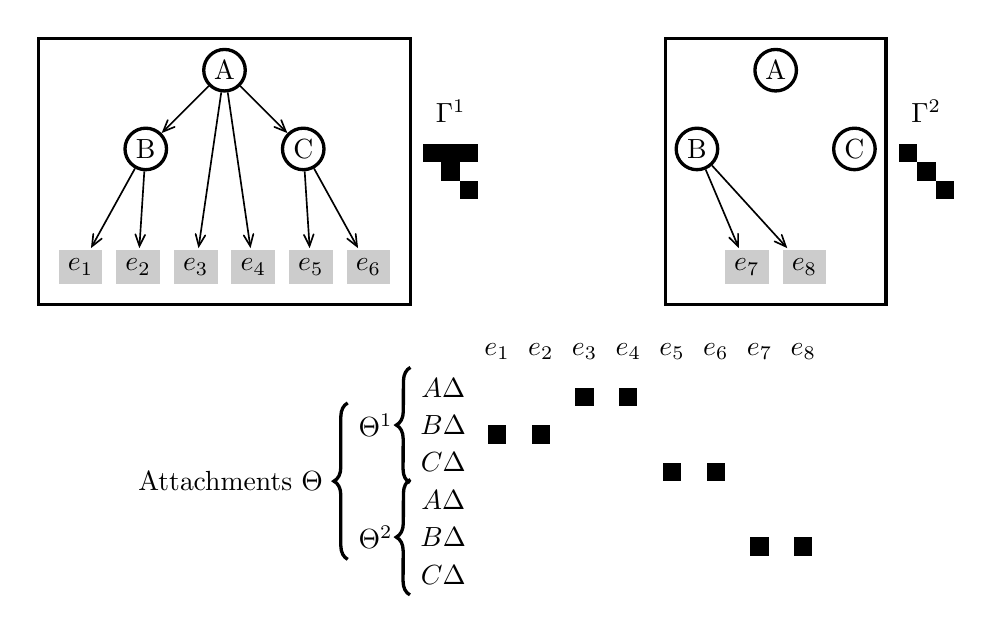
\begin{tikzpicture}[very thick, ampersand replacement=\&]

 \node[var] (a1) at (0,5mm) {A};
 \node[var] (b1) at (-1cm,-5mm) {B};
 \node[var] (c1) at (1cm,-5mm) {C};
 
 \matrix (mr) [matrix of nodes, nodes={fill=black!20}, column sep=0.5em] at (0,-2cm) {
   $e_1$ \& $e_2$ \& $e_3$ \& $e_4$ \& $e_5$ \& $e_6$ \\
 };

 \begin{scope}[shift={(7cm,0)}]
  \node[var] (a2) at (0,5mm) {A};
  \node[var] (b2) at (-10mm,-5mm) {B};
  \node[var] (c2) at (10mm,-5mm) {C};

  \matrix (ml) [matrix of nodes, nodes={fill=black!20}, column sep=0.5em] at (0,-20mm) {
   $e_7$ \& $e_8$ \\
  };
  
 \end{scope}
 
 \draw[link] (a1) to (b1);
 \draw[link] (a1) to (c1);
 
 \draw[link] (b1) to (mr-1-1);
 \draw[link] (b1) to (mr-1-2);
 \draw[link] (a1) to (mr-1-3);
 \draw[link] (a1) to (mr-1-4);
 \draw[link] (c1) to (mr-1-5);
 \draw[link] (c1) to (mr-1-6);
 \draw[link] (b2) to (ml-1-1);
 \draw[link] (b2) to (ml-1-2);
 
 \node[draw, fit=(a1) (b1) (c1) (mr)] (context1) {};
 \node[draw, fit=(a2) (b2) (c2) (ml)] (context2) {};
 \node[fit=(context1) (context2)] (ghost) {};

 \uncover<2->{
  \matrix[matrix of nodes, anchor=west] (gamma1) at (context1.east) {
   |[fill]| \& |[fill]| \& |[fill]| \\
    \& |[fill]| \&  \\
    \&  \& |[fill]| \\
  };
  \node[anchor=south] at (gamma1.north) {$\Gamma^1$};

  \matrix[matrix of nodes, anchor=west] (gamma2) at (context2.east) {
   |[fill]| \&  \&  \\
    \& |[fill]| \&  \\
    \&  \& |[fill]| \\
  };
  \node[anchor=south] at (gamma2.north) {$\Gamma^2$};
 }
 
 \uncover<3->{
 \matrix (mx) [matrix of nodes, fill=white, nodes ={black}] at (5cm,-45mm) {
  \& $e_1$ \& $e_2$ \& $e_3$ \& $e_4$ \& $e_5$ \& $e_6$ \&  $e_7$ \& $e_8$ \\
  $A\Delta$ \& \& \& |[fill=black]| \& |[fill=black]| \\
  $B\Delta$ \& |[fill=black]| \& |[fill=black]| \\
  $C\Delta$ \& \& \& \& \& |[fill=black]| \& |[fill=black]| \& \& \\
  $A\Delta$ \\
  $B\Delta$ \& \& \& \& \& \& \& |[fill]| \& |[fill]| \\
  $C\Delta$ \\
 };

 \draw[decorate,decoration={brace,mirror,amplitude=0.5em}] (mx-2-1.north west) -- (mx-4-1.south west) node[black,midway,xshift=-1.25em] (t1) {$\Theta^1$}; 

 \draw[decorate,decoration={brace,mirror,amplitude=0.5em}] (mx-5-1.north west) -- (mx-7-1.south west) node[black,midway,xshift=-1.25em] (t2) {$\Theta^2$}; 

 \draw[decorate,decoration={brace,mirror,amplitude=0.5em}] (t1.north west) -- (t2.south west) node[black,midway,anchor=east,xshift=-0.5em] {Attachments $\Theta$}; 
 
 }


\end{tikzpicture}
\end{frame}

%%% FRAMEBREAK %%%

\begin{frame}{Likelihood formulation}
\[
 \underbrace{
  L_\text{CSNEM}(\Gamma^1, \ldots, \Gamma^k, \Theta^1, \ldots, \Theta^k)
 }_{\text{CSNEM Likelihood}}
 = \prod_{i=1}^k
 \underbrace{
  L_\text{NEM}(\Gamma^i, \Theta^i)
 }_{\text{NEM Likelihood}}
\]
\pause

{\small \textcite{tresch2008structure}:}
\[
\log L_\text{NEM}(\Gamma^i, \Theta^i) = \sum_{(a,e) \in \mathcal A \times \mathcal E} \log \mathbb P ( D_{ae} | (\Gamma^i \Theta^i)_{ae} ) \pause = \mathsf{tr} ( \Gamma^i \Theta^i R^T ) + c
\]
\begin{center}\small
$R=$ log likelihood ratio matrix: $R_{ae} = \log \frac{ \mathbb P( D_{ae} | H_1 ) }{ \mathbb P( D_{ae} | H_0 ) }$
\end{center}
\pause
\[ \vdots \]
\[
\log L_\text{CSNEM}(\Gamma^1, \ldots, \Gamma^k, \Theta^1, \ldots, \Theta^k) = \mathsf{tr}( \Gamma \Theta R^{*T} ) + c^*
\]
\end{frame}

%%% FRAMEBREAK %%%

\begin{frame}{CSNEM Log Likelihood}
\begin{multline*}
\log L_\text{CSNEM}( \Gamma^1, \ldots, \Gamma^k, \Theta^1, \ldots, \Theta^k )
 = \\ \mathrm{tr}\left(
 \underbrace{\begin{bmatrix}
	\Gamma^1 & 0 & \cdots & 0 \\
	0 & \Gamma^2 & & \vdots \\
	\vdots & & \ddots & 0 \\
	0 & \cdots & 0 & \Gamma^k
 \end{bmatrix}}_{\text{Block diagonal } \Gamma}
 \underbrace{\begin{bmatrix}
	\Theta^1 \\
	\Theta^2 \\
	\vdots \\
	\Theta^k
 \end{bmatrix}}_{\text{``Big'' } \Theta; (|\mathcal A|k \times |\mathcal E|)}
 \underbrace{\begin{bmatrix}
	R^T & R^T & \cdots & R^T
 \end{bmatrix}}_{k \text{ copies}} \right) + c
\end{multline*}
\end{frame}

\begin{frame}{Learning approach}
Use MC-EMiNEM \parencite{niederberger2012mc} to solve the modified NEM learning problem.
\[
\log L( \Gamma \Theta ) + \underbrace{\sum_{(a,b) \in \mathcal A \times \mathcal A} \log \mathbb P(\Gamma_{a,b})}_{\text{edge-wise prior}} + \log \mathbb P( \Theta )
\]
\vfill
Bioconductor R package: \texttt{nem} \parencite{frohlich2008analyzing}
\end{frame}

%%% FRAMEBREAK %%%

% Maybe talk about how the simulation works
% > Mixture of random networks (varying density and k)
% > Beta parameter for noise

\begin{frame}{Evaluation on simulated data}
 \pause
 \begin{tikzpicture}
  \node (nakt) at (0mm,20mm) {$n_\mathcal{A}, k_\text{true}$};
  
  \pause
  
  \node[text block] (gs) at (0,0) {Random $\Gamma_1, \ldots, \Gamma_{k_\text{true}}$};
  \draw[link] (nakt) to (gs);
  
  \pause

  \node (theta) at (20mm, 10mm) {Random $\Theta$};
  \node[text block] (tnet) at (40mm,0) {Generating CSNEM};
  \draw[link] (gs) to (tnet);
  \draw[link,out=270,in=180] (theta) to (tnet);
  
  \pause
  
  \node[text block] (tf) at (80mm, 0) {True effect matrix};%{$F_\text{true}$};
  \draw[link] (tnet) to (tf);

  \pause
  
  \node (beta) at (70mm,-10mm) {Noise $\beta$};
  \node[text block] (lrm) at (80mm,-20mm) {$R$};
  \draw[link] (tf) to (lrm);
  \draw[link,out=0,in=90] (beta) to (lrm);

  \pause  
  
  \node (kl) at (90mm,-30mm) {$k_\text{learning}$};
  \node[text block] (lnet) at (80mm,-40mm) {Learned CSNEM};
  \draw[link] (lrm) to (lnet);
  \draw[link,out=180,in=90] (kl) to (lnet);  
  
  \pause
  
  \node[text block,text width=3cm] (lgs) at (40mm,-40mm) {Learned $\Gamma_1,\ldots,\Gamma_{k_\text{learning}}$};
  \draw[link] (lnet) to (lgs);
  
  \pause
  \node (cmpg) at (40mm,-20mm) {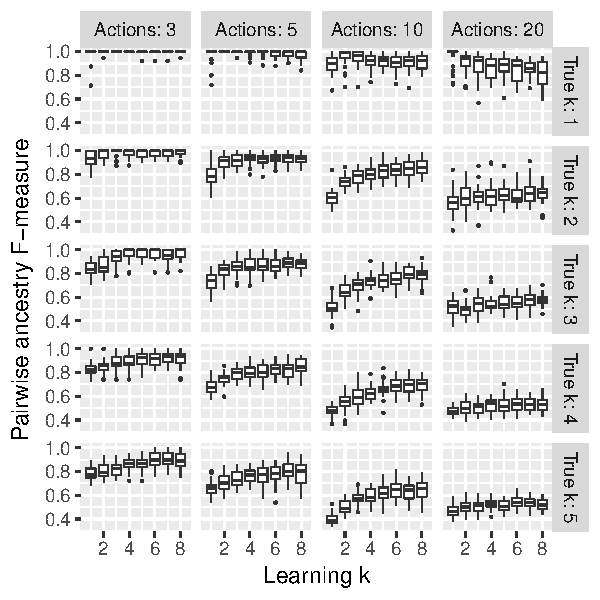
\includegraphics[width=2cm]{ancestries-f-measures.pdf}};
  \draw[link] (lgs) to (cmpg);
  \draw[link] (gs) to (cmpg);
  
  \pause
  \node[text block] (lf) at (110mm,-40mm) {Learned effect matrix};%{$F_\text{learned}$};
  \draw[link] (lnet) to (lf);
  
  \pause
  \node (cmpf) at (110mm,-15mm) {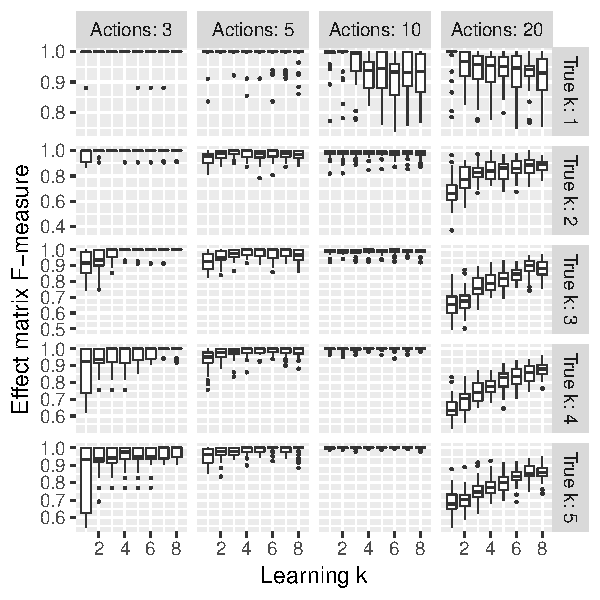
\includegraphics[width=2cm]{effect-f-measures.pdf}};
  \draw[link] (tf) to (cmpf);
  \draw[link] (lf) to (cmpf);
  
 \end{tikzpicture}
\end{frame}

%%% FRAMEBREAK %%%

\begin{frame}{Evaluation on simulated data}
$n_\mathcal{A}=20; k_\text{true}=3;$ low noise ($\beta=10$)

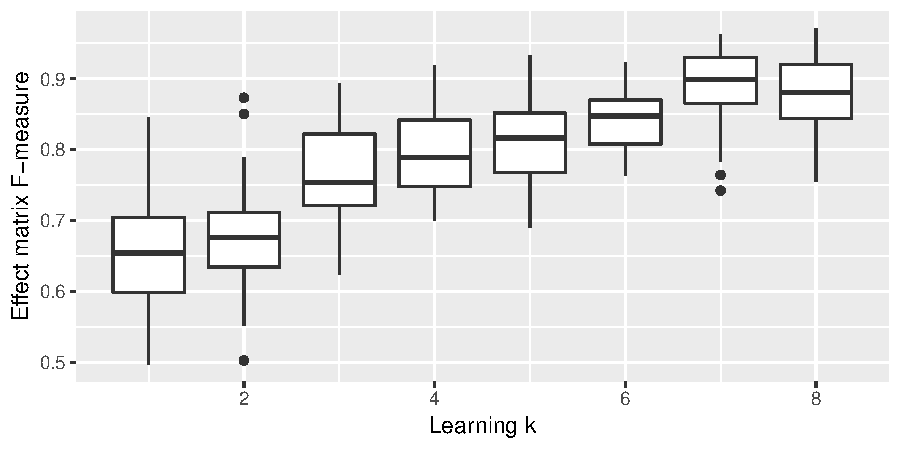
\includegraphics[width=\textwidth]{effect-for-pres.pdf}
\end{frame}

%%% FRAMEBREAK %%%

\begin{frame}{Saccharomyces cerevisiae salt stress data}
\begin{itemize}
 \item Wild type strains and 28 single-gene knockout strains
 \item Gene expression measured by microarray
  \begin{itemize}
   \item \normalsize Measurement without salt treatment
   \item \normalsize Measurement 30 minutes after 0.7 M NaCl treatment
  \end{itemize}
 \item Change in response:
\end{itemize}
\[
 \log_2 \left( \frac{\Delta \text{ strain treated}}{\Delta \text{ strain untreated}} \bigg/ \frac{\text{WT strain treated}}{\text{WT strain untreated}} \right)
\]
\vfill
{\parencite{berry2008stress, lee2011dynamic} \\}
\end{frame}

%%% FRAMEBREAK %%%

\begin{frame}{Network learned from the \textit{S. cerevisiae} data}
  \vskip5mm
  \begin{tikzpicture}
   \node[anchor=north west,inner sep=0,clip] at (-10mm,10mm) {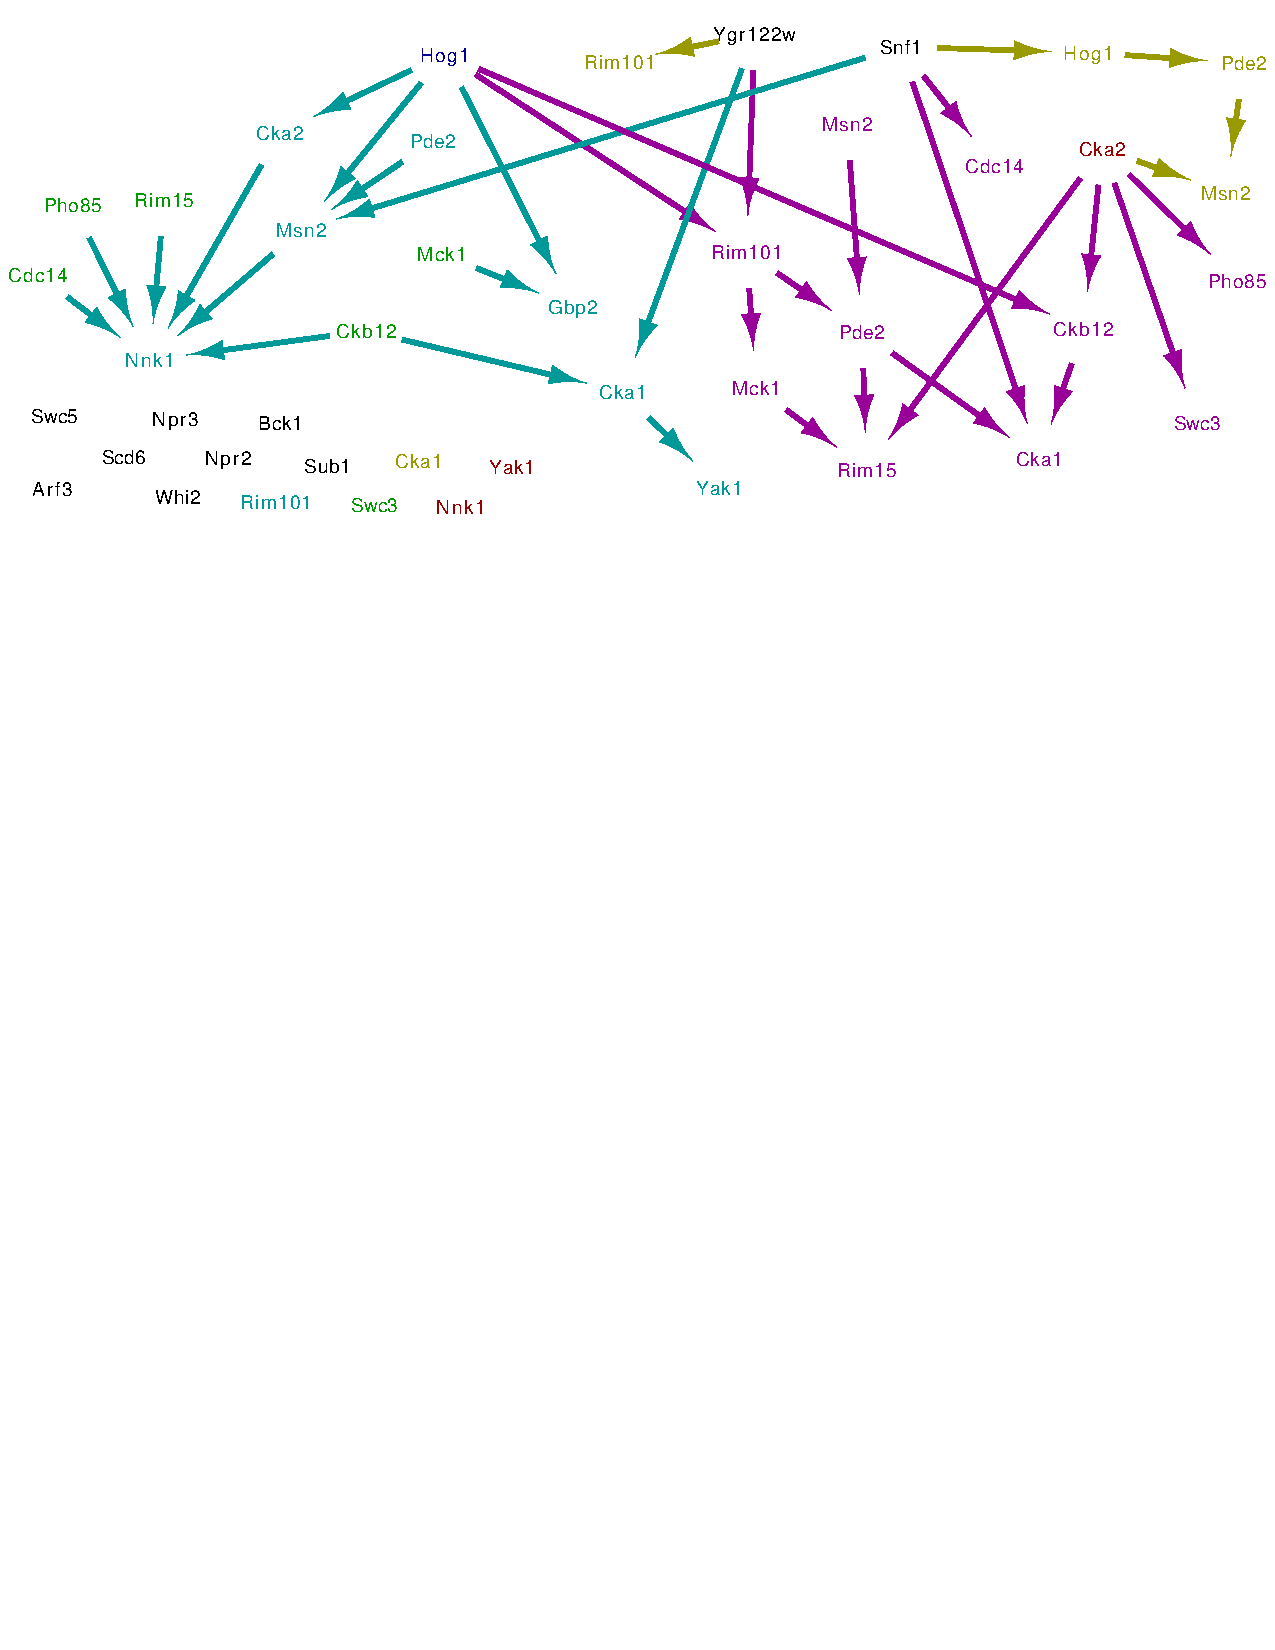
\includegraphics[width=14cm]{recomb-2018-short-names.pdf}};
   
   %\draw[help lines] (-1cm,1cm) grid (13cm,-5cm);
    
   \uncover<2>{
    \path [fill=white,opacity=0.75,even odd rule]
      (-1cm,1cm) rectangle (13cm,-5cm)
      (38.7mm,4mm) circle[radius=5mm]; %Hog1

    \draw[very thick] (38.7mm,4mm) circle[radius=5mm]; %Hog1
      
    \node[text block, text width=8cm] at (6cm,-3cm) {Hog1 is a master regulator of osmotic stress response \scriptsize \parencite{nadal2015osmostress}};
   }
   
   \uncover<3>{
    \path[fill=white,opacity=0.75,even odd rule]
      (-1cm,1cm) rectangle (13cm,-5cm)
      (38.7mm,4mm) circle[radius=5mm] %Hog1
      (20.7mm,-4.5mm) circle[radius=5mm] %Cka2
      (109mm,-26mm) circle[radius=5mm] %Ckb12
      (104mm,-40.8mm) circle[radius=5mm]; %Cka1
      
    \draw[very thick]
      (38.7mm,4mm) circle[radius=5mm] %Hog1
      (20.7mm,-4.5mm) circle[radius=5mm] %Cka2
      (109mm,-26mm) circle[radius=5mm] %Ckb12
      (104mm,-40.8mm) circle[radius=5mm]; %Cka1
    
    \node[text block, text width=8cm] at (35mm,-4cm) {Hog1 and CK complex subunits (Cka2, Ckb1/2) interact, regulate overlapping sets of genes \scriptsize
    \parencite{chasman2014pathway}};  
   }
   
   \uncover<4>{
    \path[fill=white,opacity=0.75,even odd rule]
      (-1cm,1cm) rectangle (13cm,-5cm)
      (38.7mm,4mm) circle[radius=5mm] %Hog1
      (37.5mm,-6mm) circle[radius=5mm] %Pde2
      (23mm,-15mm) circle[radius=5mm] %Msn2
      (89mm,5mm) circle[radius=5mm] %Snf1
      (109mm,4mm) circle[radius=5mm]
      (125mm,3mm) circle[radius=5mm]
      (125mm,-11mm) circle[radius=5mm];
      
    \draw[very thick]
      (38.7mm,4mm) circle[radius=5mm] %Hog1
      (37.5mm,-6mm) circle[radius=5mm] %Pde2
      (23mm,-15mm) circle[radius=5mm] %Msn2
      (89mm,5mm) circle[radius=5mm] %Snf1
      (109mm,4mm) circle[radius=5mm]
      (125mm,3mm) circle[radius=5mm]
      (125mm,-11mm) circle[radius=5mm];
   
    \node[text block, text width=8cm] at (60mm,-4cm) {Msn2 is regulated by Hog1, Pde2, and Snf1, and Pde2 plays a more significant role in regulating Msn2 during salt stress
    \scriptsize \parencite{chasman2014pathway,
     lee2008yeast,%18793336, 
mayordomo2002convergence,%12093809,
petrenko2013noise,%23615444]
rep2000transcriptional%[PMID:  10722658,
    }};  
   }

   \uncover<5>{
    \path [fill=white,opacity=0.75,even odd rule]
      (-1cm,1cm) rectangle (13cm,-5cm)
      (73mm,6mm) circle[radius=5mm] %ygr122w
      (58mm,3mm) circle[radius=5mm] %rim101 (yellow)
      (72mm,-18mm) circle[radius=5mm] %rim101 (magenta)
      ;
      
    \draw[very thick]
      (73mm,6mm) circle[radius=5mm] %ygr122w
      (58mm,3mm) circle[radius=5mm] %rim101 (yellow)
      (72mm,-18mm) circle[radius=5mm] %rim101 (magenta)
      ;
      
    \node[text block, text width=8cm] at (60mm,-4cm) {YGR122W is required for processing Rim101};  
   }
     
   \path pic {colormap};
  \end{tikzpicture}
\end{frame}

%%% FRAMEBREAK %%%

\begin{frame}{Effect group GO term enrichments}
\centering
\begin{tikzpicture}
 \node[anchor=north west,inner sep=0,clip] at (-6cm,4cm) {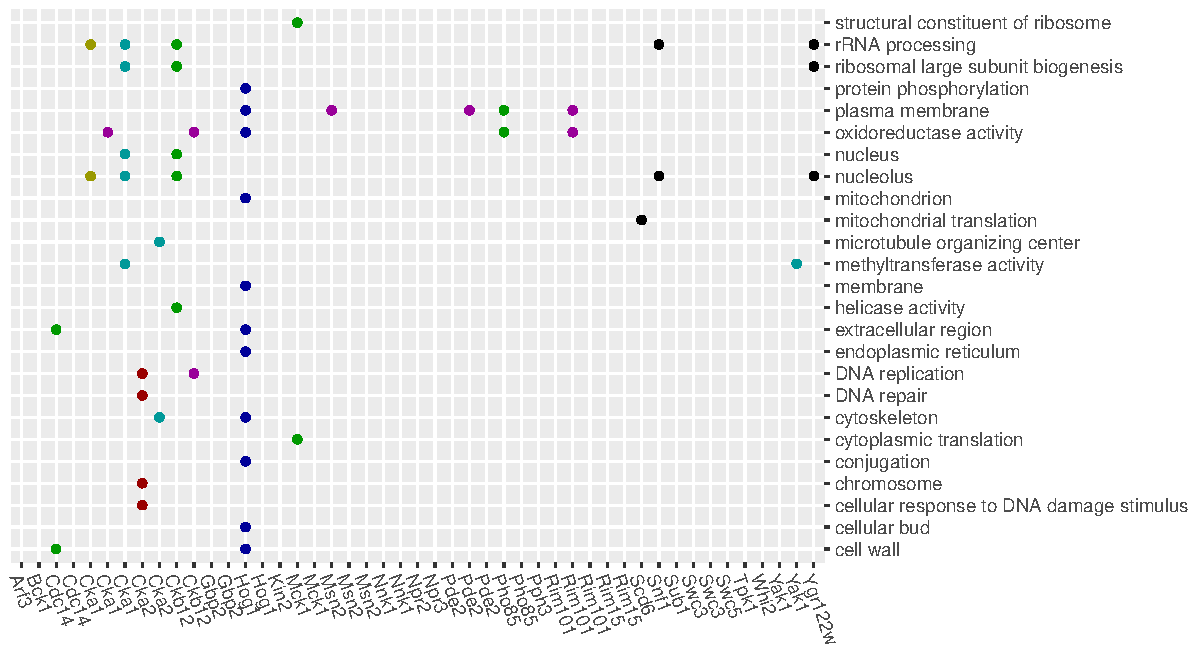
\includegraphics[width=0.8\textwidth]{go-terms-csnem-presentation}};
 \path pic {colormap};
 %\draw[help lines] (-5cm,-5cm) grid (5cm,5cm);
\end{tikzpicture}
\end{frame}

\begin{frame}{Effect group GO term enrichments}
\centering
\begin{tikzpicture}
 \node[anchor=north west,inner sep=0,clip] at (-8cm,5cm) {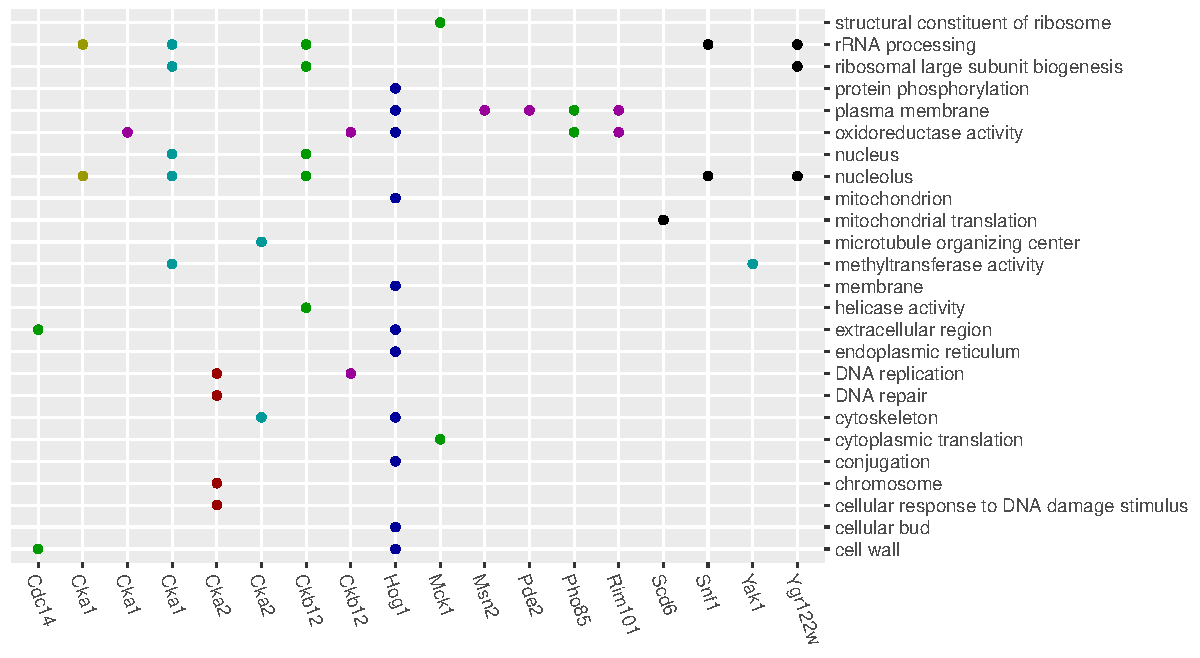
\includegraphics[width=0.95\textwidth]{go-terms-dense-csnem-presentation}};

 \draw<2>[ActionRed, very thick] (-73mm,-23mm) rectangle (-58.5mm,49.5mm);
 \draw<2>[ActionRed, very thick] (-48.5mm,-23mm) rectangle (-38.5mm,49.5mm);
 \draw<2>[ActionRed, very thick] (-79mm,29mm) -- (25mm,29mm);
  
 \draw<3>[ActionRed, very thick] (-58.5mm,-23mm) rectangle (-48.5mm,49.5mm);
 \draw<3>[ActionRed, very thick] (-79mm,2.4mm) -- (25mm,2.4mm);
 \draw<3>[ActionRed, very thick] (-79mm,22mm) -- (40mm,22mm);
  
 \path pic {colormap};
% \draw[help lines] (-8cm,5cm) grid (5cm,-2.5cm);
\end{tikzpicture}
\end{frame}

%%% FRAMEBREAK %%%

\begin{frame}{Context-wise GO term enrichments}
 \begin{tikzpicture}
  \node[anchor=south east,inner sep=0] at (1cm,-1cm) {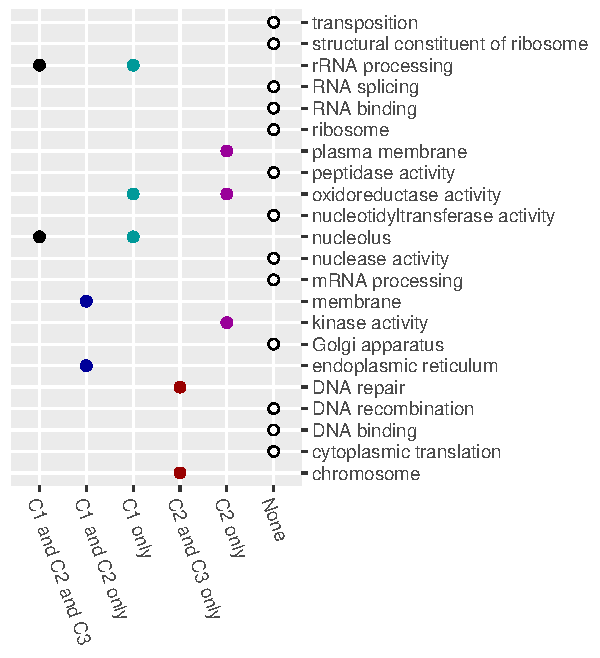
\includegraphics[scale=0.7]{go-terms-contexts-presentation}};

  \begin{scope}[ActionRed, very thick]
   \draw[link] (20mm,11.7mm) -- (-10mm,11.7mm);
   \draw[link] (20mm,25mm) -- (-1mm,25mm);
   \draw[link] (20mm,32mm) -- (-11mm,32mm);
   \draw[link] (20mm,40mm) -- (-11.5mm,40mm);
   \draw[link] (20mm,50mm) -- (-5mm,50mm);
   
   \node at (50mm,35mm) {\large Location GO terms};
  \end{scope}
  
  \path pic {colormap};
  %\draw[help lines] (0cm,0cm) grid (-5cm,6cm);
 \end{tikzpicture}
\end{frame}

%%% FRAMEBREAK %%%

\begin{frame}{Conclusions}
 \begin{itemize}
  \item We introduce a novel approach to modeling context-specific biological interactions.
  \pause
  \item Simulations show that
  \begin{itemize}
   \item context-specificity is recoverable, and
   \item a context-specific model is necessary when the data-generating process is context-specific.
  \end{itemize}
  \item Application to salt-stress data shows
  \begin{itemize}
   \item context-specific effect groups are enriched for meaningful GO categories, and
   \item the learned CSNEM aligns with known biology.
  \end{itemize}
 \end{itemize}
 \pause
 \begin{block}{Acknowledgments}
   \scriptsize
   \color{UWRed}
   NIH/NLM grant T15 LM0007359, NIH/NIAID grant U54 AI117954, and NIH/NIGMS grant R01 GM083989.
%   CIBM, Grant T15 LM0077359 from the National Library of Medicine, National~Institutes~of~Health
 \end{block}
\end{frame}

%%% FRAMEBREAK %%%
%
%\begin{frame}{Synthesis and identifiability}
%\centering
%\begin{tikzpicture}[very thick, ampersand replacement=\&]
%	\node (n) at (9em, 8em) {\begin{tikzpicture}
%		\matrix (n1) [matrix of nodes, row sep=0.5em] {
%			Hog1 \& \\
%			\& Cka2 \\
%			Ckb12 \& \\
%		};
%		\draw[->] (n1-1-1) -- (n1-2-2);
%
%		\matrix (n2) [right=of n1, matrix of nodes, row sep=0.5em] {
%			Hog1 \& \\
%			\& Cka2 \\
%			Ckb12 \& \\
%		};
%		\draw[->] (n2-1-1) -- (n2-3-1);
%		\draw[->] (n2-2-2) -- (n2-3-1);
%
%		\matrix (n3) [right=of n2, matrix of nodes, row sep=0.5em] {
%			Hog1 \& \\
%			\& Cka2 \\
%			Ckb12 \& \\
%		};
%		%\draw[->] (n3-1-1) -- (n3-3-1);
%		\node [fit=(n1),draw] {};
%		\node [fit=(n2),draw] {};
%		\node [fit=(n3),draw] {};
%	\end{tikzpicture}};
%	%\node [anchor=south east] at (n.north west) {(a)};
%	
%	\node (m) at (0,0) {\begin{tikzpicture}
%		\node (hog1) at (4em,6em) {Hog1};
%		\node (cka2) at (8em,6em) {Cka2};
%		\node (cka2-2) at (0,3em) {Cka2 [Hog1]};
%		\node (ckb12) at (10em,3em) {Ckb12}; 
%		\node (ckb12-2) at (6em,0) {Ckb12 [Hog1 Cka2]};
%		\draw[->] (hog1) -- (cka2-2);
%		\draw[->] (hog1) -- (ckb12-2);
%		\draw[->] (cka2) -- (ckb12-2);
%	\end{tikzpicture}};
%	%\node at (m.north west) {(b)};
%		
%	\node (s) at (18em, 0) {\begin{tikzpicture}
%		\node (hog1) at (0,6em) {$\{ \text{Hog1} \}$};
%		\node (cka2) at (4em,6em)  {$\{ \text{Cka2} \}$};
%		\node (ckb12) at (8em,6em) {$\{ \text{Ckb12} \}$};
%		\node (hog1-cka2) at (1em,3em) {$\{ \text{Hog1}, \text{Cka2} \}$};
%		\node (all) at (3em,0) {$\{ \text{Hog1}, \text{Cka2}, \text{Ckb12} \}$};
%		\draw[->] (hog1) -- (hog1-cka2);
%		\draw[->] (cka2) -- (hog1-cka2);
%		\draw[->] (hog1-cka2) -- (all);
%		\draw[->] (ckb12) -- (all);
%	\end{tikzpicture}};
%	%\node at (s.north west) {(c)};
%	
%\end{tikzpicture}
%\end{frame}

\end{document}